Besonders interessant wäre es gewesen die Ergebnisse einer Modalanalyse, mit denen aus einer Zeitschrittberechnung zu vergleichen. Leider konnte aber das Modell mit den Angaben aus Kapitel 13 \cite{Isemann} nicht nachgestellt werden.
Das grundlegende Vorgehen und die Ergebnisse können aber bereits entnommen werden.

Daher wird hier eine Modalanalyse mit zwei Isolationsspektren in dem Programm \emph{RStab} durchgeführt und die Ergebnisse verglichen. Denn das letztendliche Ziel soll es sein, die erzeugten Isolationsspektren in einer computergestützten Modalanalyse zur Vordimensionierung zu verwenden.

\pagebreak

\section{Beispielgebäude}
\label{sec:besipielgebaude}

Das Gebäude wurde als Mehrmassenschwinger vereinfacht modelliert. Der Fußpunkt wird dabei fest eingespannt und die Knoten der Stockwerke als nur seitlich verschieblich modelliert. Die Steifigkeiten der Stäbe betragen je

\begin{align*}
EI_z &= EI_y = 32 kN/m^2 \cdot 1238690.27 m^4\\
     &= 39638088.6 kNm^2
\end{align*}

und die Höhen und Massen der Stockwerke

\begin{table}[H]
\centering
\begin{tabular}{ |c|c|c| } 
 \hline
 - & Masse [t] & Höhe [m]\\
 \hline\hline
4. OG & 466.0 & 3.20\\
3. OG & 505.2 & 3.30\\
2. OG & 505.2 & 3.30\\
1. OG & 505.2 & 3.30\\
EG    & 505.2 & 3.30\\
 \hline \hline
$\Sigma$ & 2456.8 & 16.4\\
\hline
\end{tabular}
\end{table}

Die Parameter des Isolators zur Erzeugung der Isolationsspektren wurden wie folgt gewählt.

\makebox[1cm]{$D$}    = 0.325 m \par
\makebox[1cm]{$\mu$}  = 0.05\par
\makebox[1cm]{$m_1$}  = 2486.7 t\par
\makebox[1cm]{$m_2$}  = 1619.5 t\par
\makebox[1cm]{$k_2$}  = 32000 kN/m \par
\makebox[1cm]{$R$}    = 1.599 m\par

Daraus ergeben sich die Antwortspektren wie in \cref{fig:Isolation2}.

\pagebreak

\section{Berechnung mit RStab}
\label{sec:rstab}

In RStab wurden die Perioden und Beschleunigungen direkt eingegeben um ein benutzerdefiniertes Antwortspektrum zu erzeugen.

\begin{table}[H]
\centering
\begin{tabular}{ |c|c|c| } 
 \hline
 $T [s]$ & $S_a$ Transmissibilität $[m/s^2]$ & $S_a$ Vereinfacht $[m/s^2]$\\
 \hline\hline
0.01 & 5.6067 & 5.124\\
0.20 & 5.6346 & 5.083\\
0.40 & 5.7126 & 5.010\\
0.60 & 5.8303 & 4.945\\
0.80 & 5.9736 & 4.839\\
1.00 & 6.1238 & 4.714\\
1.20 & 6.2564 & 4.550\\
1.40 & 6.3435 & 4.396\\
1.60 & 6.3582 & 4.200\\
1.80 & 6.2816 & 3.972\\
2.00 & 6.1083 & 3.761\\
2.20 & 5.8472 & 3.475\\
2.40 & 5.5186 & 3.216\\
2.60 & 5.1478 & 2.894\\
2.80 & 4.7590 & 2.550\\
3.00 & 4.3719 & 2.280\\
3.20 & 4.0003 & 2.110\\
3.40 & 3.6527 & 1.892\\
3.60 & 3.3332 & 1.701\\
3.80 & 3.0429 & 1.457\\
4.00 & 2.7812 & 1.301\\
 \hline
\end{tabular}
\caption{Spektralbeschleunigungen der Isolationsspektren}
\end{table}

\begin{figure}[H]
    \centering
    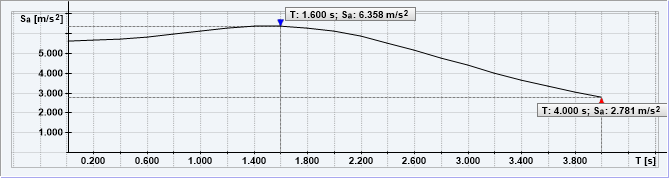
\includegraphics[width=1.0\textwidth]{RSTAB_AWS_1.png}
    \caption{Isolationsspektrum nach Ansatz der Transmissibilität in \emph{RStab}}
\end{figure}

\begin{figure}[H]
    \centering
    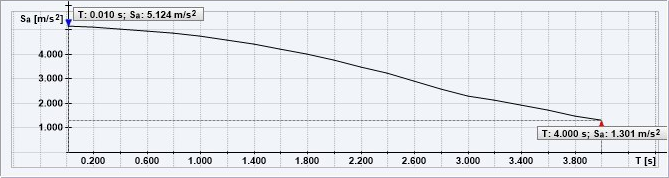
\includegraphics[width=1.0\textwidth]{RSTAB_AWS_2.png}
    \caption{Isolationsspektrum nach vereinfachtem Ansatz in \emph{RStab}}
\end{figure}

Mit dem Zusatzmodul \emph{DYNAM Pro} wurden dann Ersatzlasten in Höhe der Decken über den jeweiligen Geschossen generiert.

\begin{table}[H]
\centering
\begin{tabular}{ |c|r|r| } 
 \hline
 $-$ & $S_a$ Transmissibilität $[kN]$ & $S_a$ Vereinfacht $[kN]$\\
 \hline\hline
4. OG & 4039.2 & 3007.0\\
3. OG & 3175.4 & 2363.9\\
2. OG & 1998.2 & 1487.6\\
1. OG &  986.8 &  734.6\\
EG    &  272.5 &  202.6\\
 \hline
\end{tabular}
\caption{Ersatzlasten}
\end{table}

\pagebreak